\documentclass[11pt]{article}
\usepackage{amsmath,amssymb,amsthm}
\usepackage[numbers,sort&compress]{natbib}
\usepackage{booktabs}
\usepackage{multirow}
\usepackage{array}
\usepackage{longtable}
\usepackage{graphicx}
\usepackage{float}
\usepackage{hyperref}
\usepackage{lineno}
\usepackage{xcolor}
\usepackage{booktabs}
\usepackage{tikz}
\usetikzlibrary{arrows.meta,positioning,shapes.geometric,fit}
%\usetikzlibrary{shapes, arrows.meta, positioning}

%\journal{}
% to delete preprint ...statement

%----------------next control margins---------------------
\usepackage[
  a4paper,
  top=2.7cm,
  bottom=2.7cm,
  left=2.7cm,
  right=2.7cm
]{geometry}
%---------------------------------------
\begin{document}

\title{Mechanistic dose--response modeling in infectious diseases: a unified framework across biological scales}
\author{Ashrafur Rahman\\\small Department of Mathematics and Computer Science, College of Science \& General Studies,\\\small Alfaisal University, Riyadh, Saudi Arabia\\\small \texttt{smrahman@alfaisal.edu}}
\date{}
\maketitle
\begin{abstract}
Dose--response models connect pathogen exposure to infection risk, but classical empirical formulations and within-host mechanistic models are often presented separately. We formulate a common exposure-to-outcome representation in which dose determines an initial biological state, within-host or establishment processes generate an outcome, and variability across hosts and pathogens determines the population-level response probability. We identify how exponential and Beta--Poisson formulations, stochastic establishment models, and dynamical within-host models can be represented within this structure, while distinguishing mathematical representation from mechanistic equivalence. To illustrate the construction, we use a pathogen--immune dynamical system with heterogeneous survival and clearance parameters and estimate the probability of finite-time pathogen-burden threshold crossing across exposure doses. The resulting nonlinear response demonstrates how a population-level dose--response curve can arise through aggregation of heterogeneous within-host trajectories. The numerical example is illustrative rather than pathogen-calibrated and does not establish permanent infection. The framework provides a consistent basis for defining endpoints, locating sources of variability, and assessing when mechanistic assumptions are relevant to risk inference.
\end{abstract}
\noindent\textbf{Keywords:} Dose--response modeling; within-host dynamics; infectious disease modeling; stochastic establishment; quantitative microbial risk assessment; heterogeneity.


%\linenumbers

%------------------------------------------april 19 


%---------------end update april 23
\section{Introduction}

Dose--response relationships provide the fundamental link between pathogen exposure and infection risk, forming a central component of infectious disease modeling and quantitative microbial risk assessment (QMRA). As the probabilistic interface between exposure and infection, dose--response functions connect environmental transmission processes and within-host dynamics to population-level epidemic behavior. A key challenge is to explain how variability in exposure translates into variability in infection outcomes across hosts, pathogens, and environmental conditions. QMRA has established tractable exposure-to-risk formulations \cite{Haas2014QMRA,Schmidt2013QMRA,Hamilton2024QMRAGaps,Orahovac2026QMRABibliometric}, while challenge studies demonstrate substantial heterogeneity in infectivity \cite{Teunis2008Norovirus,DuPont1995Crypto,Chappell2006Crypto}. In parallel, within-host modeling shows that infection outcomes depend not only on dose but also on stochastic establishment, pathogen replication, immune-mediated clearance, and ecological interactions within the host \cite{Mideo2008WithinHost,Alizon2009VirulenceReview,Smith2011StochasticViruses}.

Despite these advances, dominant dose--response formulations remain classical empirical models, particularly the exponential and Beta--Poisson families \cite{Buchanan2000doseewsponse,Teunis1999GastroenteritisDose}. While analytically convenient, their parameters lack direct biological interpretation, limiting insight into how infection risk varies across hosts, pathogens, and exposure conditions, and constraining their integration with mechanistic models of transmission dynamics. Extensions incorporating heterogeneity improve flexibility but do not resolve this limitation \cite{Teunis2000BetaPoissonNotSingleHit,Haas2002DoseResponse,Xie2016GeneralizedBetaPoisson}.

Experimental and theoretical studies indicate that exposure dose alone is insufficient to explain infection outcomes. Following exposure, pathogens encounter sequential biological barriers---including gastric inactivation, epithelial defenses, microbiota-mediated competition, and immune responses---that generate nonlinear effects such as thresholds, inoculum dependence, and strong host variability \cite{Thaiss2016Microbiome,Postler2020Microbiome,Moore2020InoculumImmune}. These processes introduce stochasticity, particularly at low doses, where infection is governed by probabilistic establishment rather than average behavior. From an epidemic perspective, such nonlinearities and stochastic effects can substantially influence transmission probabilities and outbreak dynamics.

Mechanistic dose--response modeling addresses this limitation by representing the processes linking exposure to infection and deriving dose--response behavior from system dynamics. This approach enables analysis of host heterogeneity, stochastic establishment, threshold behavior, and intervention effects \cite{Rahman2018AdvancingRiskAssessment,Gostic2019Leptospira,Abe2021CampyNewDoseResponse}. Advances in Bayesian inference, identifiability analysis, and data-driven modeling further support calibration from limited or heterogeneous data \cite{Gutting2013,Sunnaker2013ABCReview,Toni2009ABC}. Importantly, mechanistic formulations provide a pathway to embed biologically grounded infection processes within epidemic models, improving the interpretation and prediction of transmission outcomes under varying exposure conditions.

However, existing approaches remain conceptually fragmented across QMRA, within-host dynamics, stochastic formulations, and hybrid models \cite{Hamilton2024QMRAGaps,Handel2015CrossingScale}. This fragmentation limits interpretability, hinders cross-scale integration, and constrains the development of predictive and transferable models for infectious disease dynamics.

This work addresses this gap by developing a unified mathematical formulation
that links exposure to infection outcomes across biological scales. The
proposed framework connects dose-to-state mapping, stochastic establishment,
within-host dynamics, biological variability, uncertainty propagation, and
population-level aggregation within a single structure.  Within this formulation, classical models arise as reduced representations of underlying stochastic and dynamical processes, while mechanistic and hybrid models provide higher-resolution descriptions. By explicitly linking exposure-driven infection processes to epidemic-scale outcomes, the framework provides a basis for integrating dose--response modeling into broader infectious disease dynamics.

The primary contribution of this work is not the development of a new pathogen-specific dose--response model, but the identification of a common mathematical structure underlying classical empirical models, stochastic establishment formulations, mechanistic within-host systems, and emerging hybrid approaches. Figure~\ref{fig:unified_mechanistic_framework} summarizes this perspective by linking exposure pathways, pathogen diversity, within-host processes, and modeling paradigms across scales. By connecting these components through a common mechanistic mapping from exposure to infection outcome, the framework provides a coherent basis for interpreting and extending dose–response models, in which observed relationships emerge from underlying biological processes and variability. A computational realization in Section~\ref{sec:illustrative_example} demonstrates how the mapping generates a finite-time threshold-crossing dose--response curve under heterogeneous within-host parameters.

%The primary contribution of this work is not the development of a new pathogen-specific dose-response model, but the identification of a common mathematical structure underlying classical empirical models, stochastic establishment formulations, mechanistic within-host systems, and emerging hybrid approaches.
%
%Figure~\ref{fig:unified_mechanistic_framework} summarizes this perspective by linking exposure pathways, pathogen diversity, within-host processes, and modeling paradigms across scales. By connecting these components through a common mechanistic mapping from exposure to infection outcome, the framework provides a coherent basis for interpreting and extending dose--response models, in which observed relationships emerge from underlying biological processes and variability. A consolidated example is presented in the computational demonstration to illustrate the unified framework.


%This work is intended as a conceptual and methodological synthesis that provides a unifying framework for integrating dose--response processes into infectious disease modeling, rather than as a pathogen-specific modeling study.

%%%%%%%%%%%%%%%%%%
\begin{figure}[t]
\centering
\resizebox{\textwidth}{!}{%
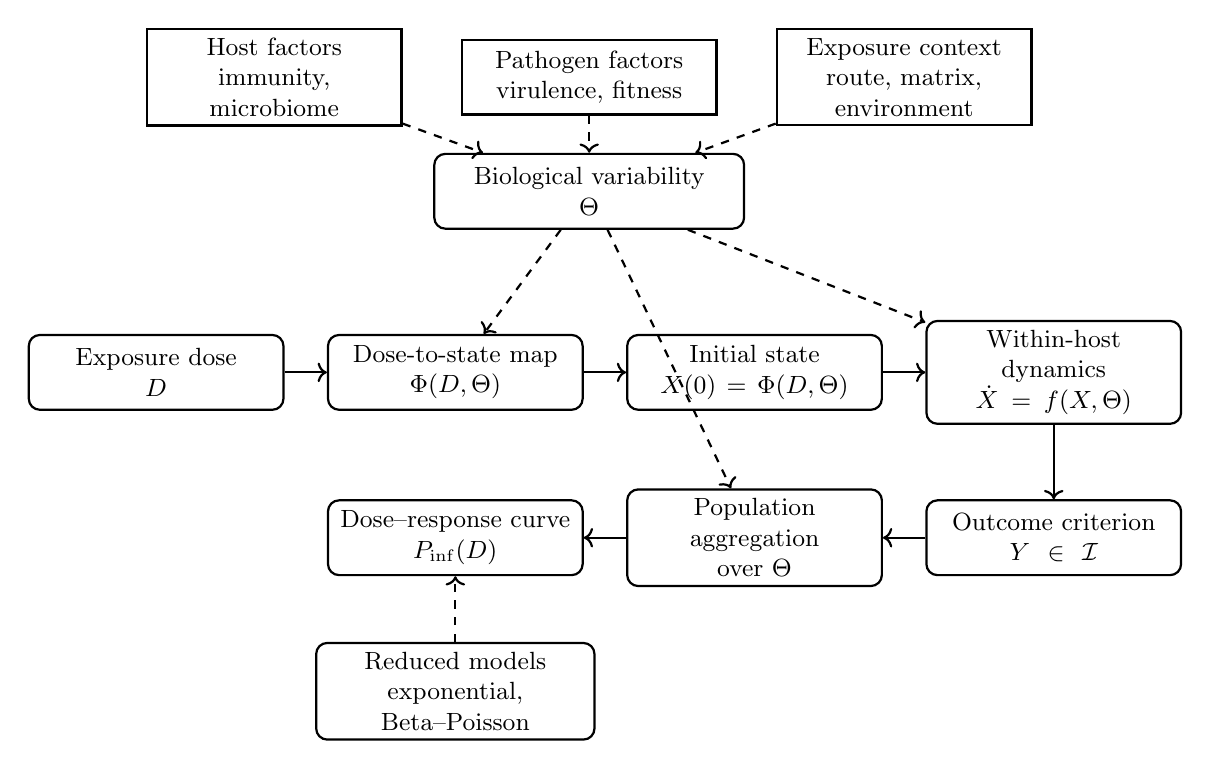
\begin{tikzpicture}[
    font=\small,
    box/.style={
        rectangle,
        rounded corners,
        draw=black,
        thick,
        align=center,
        text width=3.0cm,
        minimum height=0.95cm
    },
    source/.style={
        rectangle,
        draw=black,
        thick,
        align=center,
        text width=3.0cm,
        minimum height=0.95cm
    },
    smallbox/.style={
        rectangle,
        rounded corners,
        draw=black,
        thick,
        align=center,
        text width=3.00cm,
        minimum height=0.95cm
    },
    title/.style={
        align=center,
        font=\small\bfseries
    },
    arrow/.style={->, thick},
    dashedarrow/.style={->, thick, dashed}
]

% Sources of variability
\node[source] (host) at (0,4.3) {Host factors\\immunity, microbiome};
\node[source] (pathogen) at (4.0,4.3) {Pathogen factors\\virulence, fitness};
\node[source] (env) at (8.0,4.3) {Exposure context\\route, matrix, environment};

% Biological variability
\node[box, text width=3.7cm] (theta) at (4.0,2.85) {Biological variability\\$\Theta$};

% Pathway title
%\node[title] at (4.0,1.55) {Mechanistic pathway};

% Main mechanistic pathway
\node[box] (dose) at (-1.5,0.55) {Exposure dose\\$D$};
\node[box] (mapping) at (2.3,0.55) {Dose-to-state map\\$\Phi(D,\Theta)$};
\node[box] (initial) at (6.1,0.55) {Initial state\\$X(0)=\Phi(D,\Theta)$};
\node[box] (dynamics) at (9.9,0.55) {Within-host dynamics\\$\dot X=f(X,\Theta)$};

% Outcome and aggregation
\node[box] (event) at (9.9,-1.55) {Outcome criterion\\$Y\in\mathcal I$};
\node[box] (aggregation) at (6.1,-1.55) {Population aggregation\\over $\Theta$};
\node[box] (risk) at (2.3,-1.55) {Dose--response curve\\$P_{\mathrm{inf}}(D)$};

% Reduced classical models
\node[smallbox, text width=3.3cm] (classical) at (2.3,-3.5)
{Reduced models\\exponential, Beta--Poisson};

% Main process arrows
\draw[arrow] (dose) -- (mapping);
\draw[arrow] (mapping) -- (initial);
\draw[arrow] (initial) -- (dynamics);
\draw[arrow] (dynamics) -- (event);
\draw[arrow] (event) -- (aggregation);
\draw[arrow] (aggregation) -- (risk);

% Variability arrows
\draw[dashedarrow] (host) -- (theta);
\draw[dashedarrow] (pathogen) -- (theta);
\draw[dashedarrow] (env) -- (theta);

\draw[dashedarrow] (theta) -- (mapping);
\draw[dashedarrow] (theta) -- (dynamics);
\draw[dashedarrow] (theta) -- (aggregation);

% Classical reduced-model connection
\draw[dashedarrow] (classical) -- (risk);

\end{tikzpicture}%
}

\caption{
Unified mechanistic framework for dose--response modeling. Exposure dose $D$ is mapped to an initial within-host state through $\Phi(D,\Theta)$, where $\Theta$ represents biological variability in host, pathogen, and exposure conditions. Within-host dynamics generate trajectories that are classified according to an outcome criterion $\mathcal I$. Population-level dose--response relationships emerge by aggregating trajectory-level outcomes across heterogeneous biological conditions. Classical, stochastic, mechanistic, and hybrid dose--response models can be interpreted as alternative realizations of this broader exposure-to-outcome framework.
}
\label{fig:unified_mechanistic_framework}
\end{figure}

%%%%%



\section{Scope and Structure}

This methodological study develops an exposure-to-outcome representation and evaluates its construction through an illustrative within-host simulation. The selected literature establishes the assumptions and relationships of existing model classes; it is not intended as a systematic review.

The literature considered spans classical empirical dose--response models, mechanistic formulations derived from within-host dynamics, and recent extensions incorporating stochasticity, multiscale coupling, and data-driven inference. Emphasis is placed on identifying common structural elements across these approaches and clarifying how different modeling frameworks relate to one another. This perspective is illustrated schematically in Figure~\ref{fig:unified_mechanistic_framework}, which highlights the key components linking exposure, biological processes, and population-level risk.

The paper is organized as follows. Section~\ref{sec:classical_to_mechanistic} reviews classical dose--response models and their underlying assumptions, and introduces their extension toward stochastic and within-host interpretations. Section~\ref{sec:mechanistic_framework} develops a mechanistic framework that links within-host dynamics to infection probability and explains how dose--response relationships emerge from biological processes. Section~\ref{sec:extensions} presents extensions of this framework, including stochastic, spatial, and hybrid modeling approaches. Section~\ref{sec:challenges_future} discusses key challenges and future directions, including identifiability, data integration, and computational methods. Section~\ref{sec:illustrative_example} presents the computational demonstration of the unified framework. Finally, Section~\ref{sec:conclusion} concludes the paper.


%--------------------------------------------------------------------------------------
\section{From Classical Models to Mechanistic Interpretation} %section 3
\label{sec:classical_to_mechanistic}

Classical dose--response models provide the standard mathematical link between pathogen exposure and infection probability in quantitative microbial risk assessment (QMRA). Their central strength is parsimony: they summarize complex exposure--response data using tractable probability functions that can be fitted from challenge, outbreak, or surveillance data \cite{Haas2014QMRA,Schmidt2013QMRA,Teunis2000BetaPoissonNotSingleHit}. However, this tractability is achieved by collapsing the biological processes between exposure and infection into a small number of effective parameters. The resulting models are therefore useful empirical summaries, but they provide limited insight into the mechanisms by which pathogens survive, establish, expand, or are cleared within the host.

This section develops the bridge from classical formulations to mechanistic interpretation. The main point is not that classical models should be discarded, but that they can be understood as reduced descriptions of underlying stochastic and dynamical processes. This interpretation clarifies both their utility and their limitations, and motivates a mechanistic framework in which dose--response relationships emerge from exposure survival, pathogen establishment, within-host expansion, and host-mediated clearance.

\begin{table*}[htbp]
\centering
\caption{From classical dose--response models to mechanistic interpretation. Classical models provide tractable exposure--risk functions, whereas mechanistic models interpret infection probability as an emergent property of biological processes.}
\label{tab:classical_mechanistic_bridge}
\resizebox{\textwidth}{!}{%
\begin{tabular}{p{3.2cm} p{3.2cm} p{3.8cm} p{3.5cm} p{3.5cm} p{4.2cm}}
\toprule
\textbf{Modeling perspective} &
\textbf{Mathematical structure} &
\textbf{Biological interpretation} &
\textbf{Strength} &
\textbf{Main limitation} &
\textbf{Representative citations} \\
\midrule

Exponential model &
$P_{\mathrm{inf}}(D)=1-e^{-rD}$ &
Independent action; each pathogen has the same effective probability of successful establishment &
Analytically simple; widely used in QMRA; interpretable as a limiting establishment process &
Assumes independence and constant infectivity; cannot represent thresholds, feedback, or host dynamics &
\cite{Haas2014QMRA,Schmidt2013QMRA, Teunis2000BetaPoissonNotSingleHit} \\

Beta--Poisson model &
$P_{\mathrm{inf}}(D)=1-\left(1+D/\beta\right)^{-\alpha}$ &
Effective heterogeneity in host susceptibility and/or pathogen infectivity &
More flexible than the Exponential model; often improves fit to challenge data &
Heterogeneity is statistical rather than mechanistic; parameters remain difficult to map to biological processes &
\cite{Haas2002DoseResponse,Messner2001CryptosporidiumRisk,Teunis2000BetaPoissonNotSingleHit,Teunis2002CryptoVariation} \\

Generalized empirical models &
Approximate Beta--Poisson and related flexible formulations &
Dose--response represented as an empirical exposure--outcome curve &
Useful for applied risk estimation under limited data &
Greater flexibility does not necessarily improve biological interpretability &
\cite{Haas2002DoseResponse,Xie2016GeneralizedBetaPoisson} \\

Stochastic establishment interpretation &
$P_{\mathrm{inf}}(D)=1-(P_{\mathrm{ext}})^D$ &
Infection occurs if at least one initially introduced lineage avoids early extinction &
Connects classical models to branching and birth--death processes &
Requires assumptions about early survival and independence of lineages &
\cite{Allen2010Stochastic,Gostic2019Leptospira,Rahman2016Listeria} \\

Mechanistic dynamical systems &
ODEs or stochastic processes for pathogen growth, host response, and clearance &
Dose determines initial conditions; infection probability emerges from system trajectories &
Captures thresholds, feedback, nonlinear growth, and intervention mechanisms &
Requires more parameters, richer data, and identifiability analysis &
\cite{Mideo2008WithinHost,Murray2002MathematicalBiology1,Perelson2002ModellingViral} \\

Heterogeneous mechanistic models &
Distributed biological parameters across hosts, strains, or environments &
Variability arises from measurable differences in immune state, microbiome, virulence, or exposure conditions &
Supports biologically interpretable variability and extrapolation &
High-dimensional parameter spaces can create practical and structural identifiability problems &
\cite{NASEM2018MicrobiomeRisk,Pouillot2015Listeria,Thaiss2016Microbiome} \\

Hybrid and multiscale frameworks &
Coupled within-host, transmission, statistical, or data-driven models &
Links biological mechanisms to population-level risk and inference &
Unifies QMRA, within-host modeling, and modern data-integrated approaches &
Computationally demanding; requires careful validation and biological constraints &
\cite{Capone2022QMRAEffectMeasures,Handel2015CrossingScale,Mideo2008WithinHost} \\

\bottomrule
\end{tabular}
}
\end{table*}

\subsection{Classical formulations and their assumptions}

The Exponential model is the simplest and most widely used classical dose--response formulation:
\begin{equation}
P_{\mathrm{inf}}(D) = 1 - e^{-rD},
\label{eq:exponential}
\end{equation}
where $D$ denotes the administered or ingested dose and $r$ is an effective per-pathogen probability of successful establishment. This model follows from the independent action hypothesis, which assumes that each pathogen acts independently and has the same probability of initiating infection \cite{Haas2014QMRA,Teunis2000BetaPoissonNotSingleHit}. If the probability that a single pathogen fails to establish is $1-r$, then the probability that all $D$ pathogens fail is approximately $(1-r)^D \approx e^{-rD}$ for small $r$, yielding Eq.~\eqref{eq:exponential}.

The Beta--Poisson model relaxes the assumption of a fixed establishment probability by allowing infectivity or susceptibility to vary across hosts or exposures:
\begin{equation}
P_{\mathrm{inf}}(D) =
1 - \left(1+\frac{D}{\beta}\right)^{-\alpha},
\label{eq:betapoisson}
\end{equation}
where $\alpha$ and $\beta$ are shape parameters associated with heterogeneity in the underlying infection process \cite{Haas2014QMRA,Moore2020InoculumImmune}. This model often provides a better empirical fit than the Exponential model, especially when challenge data exhibit overdispersion or substantial host-to-host variability.

Despite their practical value, both formulations remain phenomenological. They describe how infection probability changes with dose, but they do not explicitly represent the processes that determine whether an introduced pathogen survives early barriers, establishes in a target niche, expands within the host, or is eliminated by immune responses. Consequently, classical models often have limited transportability across host populations, pathogen strains, exposure routes, or intervention scenarios \cite{Haas2014QMRA,Levin2001WithinHost,Rahman2018AdvancingRiskAssessment}.

\subsection{Classical models as reduced mechanistic descriptions}
\label{stochastic} % section 3.2
A mechanistic interpretation of classical dose--response models can be obtained by considering early infection as a stochastic establishment process. Let $N(t)$ denote the pathogen population size after exposure, and suppose that early pathogen dynamics are approximated by a birth--death process with birth rate $\lambda$ and death rate $\mu$. The extinction probability for a single introduced pathogen is
\begin{equation}
P_{\mathrm{ext}} =
\begin{cases}
1, & \lambda \leq \mu,\\[4pt]
\mu/\lambda, & \lambda > \mu.
\end{cases}
\label{eq:extinction}
\end{equation}
If $D$ introduced pathogens act independently during the earliest phase of infection, the probability that all lineages go extinct is $(P_{\mathrm{ext}})^D$. Therefore,
\begin{equation}
P_{\mathrm{inf}}(D) = 1 - \left(P_{\mathrm{ext}}\right)^D .
\label{eq:infection_extinction}
\end{equation}
When $P_{\mathrm{ext}}\approx 1-r$, Eq.~\eqref{eq:infection_extinction} reduces to the Exponential model. Thus, the Exponential dose--response curve can be interpreted as a coarse-grained approximation of stochastic establishment under independence and homogeneous infectivity.

This derivation is useful because it reframes classical models as limiting cases rather than purely empirical curves. The parameter $r$ is no longer simply a fitted constant; it can be viewed as an effective summary of early survival, niche access, pathogen replication, and host-mediated loss. Similarly, the Beta--Poisson model can be interpreted as arising when this effective establishment probability varies across hosts, pathogens, or exposure conditions. However, unless the source of that variability is explicitly modeled, the resulting parameters remain statistical summaries rather than directly measurable biological quantities.

\subsection{From dose as input to infection as a dynamical outcome} \label{dose-to-infection}
Mechanistic dose--response models extend this interpretation by explicitly representing the biological processes governing infection. Within-host dynamical models capture pathogen replication, immune response, and target-cell dynamics \cite{Moore2020InoculumImmune,Vlazaki2020BacterialReview}. Dose is treated as an initial condition or input to a within-host system, while infection is defined by a dynamical outcome such as persistence, threshold crossing, tissue invasion, or failure of clearance. In abstract form,
\begin{equation}
P_{\mathrm{inf}}(D)=\Pr\left(\mathcal{E}(X(t;D))\right),
\label{eq:abstract_event}
\end{equation}
where $X(t;D)$ denotes the within-host state trajectory following exposure dose $D$, and $\mathcal{E}$ denotes an infection-establishment event.

For example, if infection is defined as pathogen burden exceeding a critical threshold $X_c$, then
\begin{equation}
P_{\mathrm{inf}}(D)
=
\Pr\left(
\max_{t\geq 0} X(t;D) \geq X_c
\right).
\label{eq:threshold_event}
\end{equation}
This formulation makes explicit that infection risk may arise from threshold crossing, stochastic extinction, nonlinear growth, immune-mediated clearance, or ecological competition within the host.

A general deterministic representation of pathogen dynamics can be written as
\begin{equation}
\frac{dN}{dt}
=
G(N,\theta_G)
-
H(N,I,\theta_H)
-
E(N,\theta_E),
\label{eq:general_mechanistic}
\end{equation}
where $G$ represents pathogen growth, $H$ represents host-mediated clearance or immune control, $I$ denotes immune activity, and $E$ represents environmental or physiological loss. In stochastic form, the same idea can be represented as
\begin{equation}
dX = f(X,I;\theta)\,dt + \sigma(X,I)\,dW_t,
\label{eq:stochastic_general}
\end{equation}
where $W_t$ is a Wiener process and $\sigma(X,I)$ controls demographic or environmental variability \cite{Allen2010Stochastic,Murray2002MathematicalBiology1}.

These formulations shift the interpretation of dose--response relationships. The curve $P_{\mathrm{inf}}(D)$ is not imposed in advance; it is generated by the distribution of system trajectories initiated by dose $D$.

\subsection{A minimal pathogen--immune framework}\label{path_immune_frame}

To make the mechanistic structure explicit, we consider a minimal within-host dynamical system that captures the essential interaction between pathogen replication and immune response \cite{Mideo2008WithinHost,Murray2002MathematicalBiology1,Perelson2002ModellingViral}. A minimal mechanistic model can be written by coupling pathogen burden $P(t)$ to immune activity $I(t)$:
\begin{align}
\frac{dP}{dt}
&=
\lambda P\left(1-\frac{P}{K}\right)
-\phi PI
-\mu P,
\label{eq:pathogen_dynamics}
\\
\frac{dI}{dt}
&=
\alpha P
+
\beta I\left(1-\frac{I}{I_{\max}}\right)
-\delta I .
\label{eq:immune_dynamics}
\end{align}
Here, $\lambda$ is the pathogen replication rate, $K$ is an ecological or tissue-level carrying capacity, $\phi$ represents immune-mediated killing, $\mu$ is baseline loss, $\alpha$ describes immune activation by pathogen burden, $\beta$ describes immune expansion, and $\delta$ represents immune decay. Together, this system represents the balance between pathogen replication and immune-mediated control, illustrating how infection outcomes can be interpreted as trajectory-dependent properties of within-host dynamics.

The external exposure dose enters through a dose-to-state mapping,
\begin{equation}
P(0)=\eta D,
\label{eq:dose_to_state}
\end{equation}
where $\eta$ summarizes survival through early barriers such as gastric acidity, mucus, environmental stress, or anatomical deposition. More detailed models may replace Eq.~\eqref{eq:dose_to_state} with multiple compartments representing stomach, intestine, tissue, or respiratory deposition sites, but the conceptual role is the same: exposure is translated into an internal initial condition.


This minimal system can generate several features that classical models cannot represent directly. Depending on parameter values and initial conditions, trajectories may lead to clearance, persistence, transient colonization, or rapid expansion. Thresholds arise as boundaries between these dynamical regimes rather than as externally imposed dose cutoffs. Host heterogeneity can be represented by distributions over parameters such as $\eta$, $\lambda$, $\phi$, $K$, or immune activation strength, allowing population-level dose--response curves to be generated by aggregating outcomes across heterogeneous hosts. The broader implications of emergent thresholds and biological heterogeneity are considered in the following subsection.

%The illustrative model highlights how dose--response relationships can emerge from within-host dynamics. In practice, however, infection outcomes are also shaped by threshold effects and biological variability across hosts, pathogens, and exposure conditions. These factors are considered in the following subsection.



\subsection{Emergent thresholds, heterogeneity, and biological interpretation}

A central implication of the mechanistic view is that thresholds are context-dependent properties of the host--pathogen system. They may arise from stochastic extinction at low dose, nonlinear immune activation, density-dependent growth, resource limitation, or Allee-type effects \cite{Antia1994ImmuneClearance,Levin2001WithinHost,Rahman2016Listeria}. Thus, a small change in dose, immune state, microbiome composition, or pathogen fitness can shift the system from clearance to establishment.

This perspective also changes how heterogeneity is interpreted. In classical models, heterogeneity is introduced statistically through parameter distributions. In mechanistic models, heterogeneity can be tied to measurable biological sources: variation in early survival, receptor availability, immune responsiveness, microbiome-mediated colonization resistance, strain virulence, or tissue-specific growth conditions \cite{NASEM2018MicrobiomeRisk,Pouillot2015Listeria,Thaiss2016Microbiome}. The resulting population-level dose--response curve is then an aggregate of biologically interpretable individual-level processes.

Mechanistic interpretation therefore provides a bridge between mathematical tractability and biological realism. Classical models remain useful when data are sparse or when the goal is routine risk estimation within observed dose ranges. Mechanistic models become essential when the goal is extrapolation, intervention analysis, host stratification, cross-species translation, or integration of multiscale data. This distinction motivates the next section, where dose--response curves are generated explicitly from within-host trajectories and population-level aggregation. 

%The formulations developed in this section establish a continuum of models linking phenomenological dose--response relationships to stochastic establishment processes and fully dynamical within-host systems. While these representations provide complementary perspectives, they share a common underlying structure in which exposure determines initial conditions, biological dynamics govern system evolution, and infection corresponds to a trajectory-dependent outcome.
%
%This observation motivates a unifying framework in which dose--response relationships are interpreted as emergent properties of mechanistic processes rather than prescribed functions. The next section formalizes this perspective by organizing these components into a coherent mapping from exposure to infection probability and population-level risk.


The formulations discussed in this section establish a
continuum from phenomenological dose--response models
to stochastic establishment processes and mechanistic
within-host systems. Their common exposure-to-outcome
structure motivates the unified mathematical framework
developed in Section~\ref{sec:mechanistic_framework}.

%Mechanistic interpretation provides a link between biological processes and observable infection outcomes, clarifying when classical models are sufficient and when more detailed representations are required. This distinction motivates the next section, where dose--response curves are generated explicitly from within-host trajectories and population-level aggregation.


%--------------------------------------------------------------------------------------
% Section 4

\section{A Mechanistic Framework for Dose--Response Modeling}
\label{sec:mechanistic_framework}

The models reviewed in Section 3 differ in mathematical structure and biological detail, yet all seek to describe the same process: how pathogen exposure leads to infection. This observation motivates a unified framework that focuses on the common exposure-to-outcome mapping underlying classical, stochastic, mechanistic, and hybrid dose--response models.

Within this perspective, dose--response relationships are not treated as direct empirical functions of dose. Instead, they emerge from the interaction of dose-to-state mapping, within-host dynamics, outcome definitions, and biological variability.% Figure~\ref{fig:unified_mechanistic_framework} summarizes this conceptual structure.

At a general level, the population-level probability of infection can be expressed as
\begin{equation}
P_{\mathrm{inf}}(D)
=
\Pr\left(
Y(\Phi(D,\Theta))
\in \mathcal I
\right),
\label{eq:unified_framework}
\end{equation}
Equation~\eqref{eq:unified_framework} generalizes the trajectory-based formulation in Eq.~\eqref{eq:abstract_event}, where $X(t;D)$ corresponds to a particular realization of the biological trajectory $Y$, and the event $E$ is represented by the outcome set $\mathcal I$. %
%
%where $D$ denotes exposure dose, $\Phi(D,\Theta)$ maps exposure to an initial within-host state, $Y$ represents the resulting biological trajectory, $\Theta$ captures biological variability, and $\mathcal I$ defines the outcome of interest. 
Equation~\eqref{eq:unified_framework} provides a common mathematical structure within which diverse dose--response models can be interpreted as alternative representations of the same underlying process as illustrated in Figure~\ref{fig:unified_mechanistic_framework}.


\begin{table*}[ht]
\centering
\caption{Mechanistic framework for dose--response modeling. Dose--response curves emerge from within-host dynamics, outcome definitions, and population-level aggregation under biological variability.}
\label{tab:mechanistic_framework_generation}
\resizebox{\textwidth}{!}{%
\begin{tabular}{p{3.2cm} p{3.5cm} p{3.6cm} p{3.5cm} p{4.2cm}}
\toprule
\textbf{Component} &
\textbf{Mathematical structure} &
\textbf{Biological interpretation} &
\textbf{Role in dose--response} &
\textbf{Representative citations} \\
\midrule

Dose-to-state mapping &
$P(0)=\eta D$ &
Survival through early barriers (gastric, environmental, anatomical) &
Links exposure to initial within-host conditions &
\cite{Abe2020CampyInvasion,Koseki2011GastricSurvival,Zhang2023Survival} \\

Within-host dynamics &
ODEs / stochastic processes &
Pathogen growth, immune response, ecological interactions &
Generates trajectories from initial conditions &
\cite{Mideo2008WithinHost,Moore2020InoculumImmune,Murray2002MathematicalBiology1,Perelson2002ModellingViral} \\

Outcome definition &
Thresholds, persistence, peak burden &
Operational definition of infection or disease &
Maps trajectories to outcomes &
\cite{Levin2001WithinHost,Moore2020InoculumImmune,Rahman2016Listeria} \\

Population variability &
Parameter distributions $\Theta$ &
Host heterogeneity, strain variability, environment &
Introduces variability across individuals &
\cite{Hamilton2024QMRAGaps,Pouillot2010,Pouillot2003Uncertainty,Teunis2002CryptoVariation} \\

Statistical aggregation &
$P_{\mathrm{inf}}(D)
=\Pr\left(
Y(\Phi(D,\Theta))
\in \mathcal I
\right)$ &
Probability of infection across heterogeneous hosts &
Produces population-level dose--response curve &
\cite{Hamilton2024QMRAGaps,Messner2001CryptosporidiumRisk} \\

%Sensitivity and identifiability &
%Sensitivity / identifiability analysis &
%Key biological drivers of infection risk &
%Links model behavior to data and inference &
%\cite{Gutting2013,Raue2009StructuralIdentifiability,Preston2025Identifiability} \\

\bottomrule
\end{tabular}
}
\end{table*}

\subsection{The Exposure-to-Outcome Mapping}


The exposure-to-outcome mapping in Eq.~\eqref{eq:unified_framework}
provides a modular representation of infection risk.
The dose-to-state map $\Phi(D,\Theta)$ determines
the initial biological state, while the within-host
model generates trajectories whose outcomes are
evaluated against the criterion $\mathcal{I}$.
Population-level risk is then obtained by
aggregating these outcomes over biological
variability represented by $\Theta$.


In this interpretation, classical models represent
reduced descriptions of the exposure-to-outcome
mapping, whereas mechanistic models explicitly
resolve one or more of its intermediate components.


%In this interpretation,
%dose--response curves are not prescribed directly but arise as
%statistical summaries of underlying biological processes. Classical
%models therefore represent reduced descriptions of this mapping,
%whereas mechanistic models explicitly resolve one or more of its
%intermediate components.



\subsection{Recovering Existing Model Classes from the Framework}

Equation~\eqref{eq:unified_framework}  reveals that classical, stochastic, mechanistic, and hybrid dose--response models differ primarily in how explicitly they represent the intermediate processes linking exposure to outcome. Within this perspective, the major classes of dose--response models can be interpreted as alternative representations of the same exposure-to-outcome mapping.

Classical dose--response models arise when the intermediate biological processes are not represented explicitly and infection probability is specified directly as a function of dose. In this case, the effects of pathogen survival, within-host dynamics, and host variability are absorbed into a small number of effective parameters, yielding a direct relationship between exposure and risk.

Stochastic establishment models introduce an explicit representation of the probability that one or more pathogen lineages survive early extinction. Infection is determined by the stochastic fate of initially introduced pathogens, while subsequent within-host dynamics remain implicit.

Mechanistic models further resolve the biological processes represented by $Y$. Exposure determines the initial state through $\Phi(D,\Theta)$, and infection emerges as a trajectory-dependent outcome of within-host dynamics. Hybrid and multiscale approaches extend this representation by combining mechanistic components with stochastic, statistical, or data-driven elements.


The relationship among the major classes of dose–response models can be organized according to their degree of biological resolution:
%The relationship among the major classes of dose--response models can be viewed as a spectrum of increasing biological resolution,

%\[
%\left\{\text{Classical}, \text{Stochastic},\text{Mechanistic}\right\} \subset
%\text{Unified Framework}.
%\]
\[
\{\text{Classical, Stochastic, Mechanistic, Hybrid}\}
\subset \text{Unified Framework}.
\]

This inclusion emphasizes that the unified framework
accommodates different levels of biological resolution
without requiring a single modeling paradigm.

%Classical models represent infection probability directly as a function of dose, stochastic models explicitly incorporate establishment processes, mechanistic models resolve within-host dynamics, and the unified framework generalizes these approaches through explicit representations of dose-to-state mapping, biological trajectories, outcome definitions, and heterogeneity. The framework therefore provides a common language for comparing models that differ substantially in biological resolution while preserving their underlying conceptual connection. %In this sense, existing dose--response models can be interpreted as alternative realizations or simplifications of a common exposure-to-outcome mapping.

\subsection{Biological Variability, Emergent Thresholds, and Uncertainty Propagation}

The unified framework provides a natural structure for distinguishing
biological variability from epistemic uncertainty and for identifying how
each influences the mapping from exposure to population-level infection risk. In
\[
P_{\mathrm{inf}}(D)
=
\Pr\!\left(Y(\Phi(D,\Theta))\in\mathcal{I}\right),
\]
variability may enter at each stage of the exposure-to-outcome mapping.
Uncertainty in the external dose affects the exposure input; uncertainty
in the dose-to-state map $\Phi$ affects the effective pathogen burden
reaching the relevant within-host compartment; uncertainty in parameters
governing $Y$ affects predicted pathogen growth, establishment, and
clearance; and uncertainty in the outcome criterion $\mathcal{I}$ affects
how trajectories are classified as infection, colonization, or disease.
Consequently, uncertainty in population-level risk is not associated with
a single model parameter, but is propagated through the complete
exposure-to-outcome mapping.

It is useful in this context to distinguish biological variability from
epistemic uncertainty. Biological variability represents genuine
differences among hosts, pathogens, and exposure conditions and is encoded
through $\Theta$. Examples include differences in host susceptibility,
immune responsiveness, pathogen virulence, microbiome composition,
exposure route, and environmental conditions. Epistemic uncertainty,
in contrast, reflects incomplete knowledge of quantities such as the
administered dose, survival fraction, model parameters, biological
mechanisms, or outcome thresholds. The former generates a distribution
of risks across heterogeneous individuals, whereas the latter limits
confidence in the estimated distribution and its population-level
summary. Maintaining this distinction is particularly important in risk
assessment, where variability and uncertainty have different
interpretations and implications for decision making
\cite{Pouillot2010,Pouillot2003Uncertainty}.

Threshold-like behavior provides an example of how these sources of
variability and uncertainty interact with the underlying dynamics.
Infection may require pathogen populations to reach levels sufficient
for persistence, invasion, or transmission. Such transitions can arise
from stochastic establishment, nonlinear within-host dynamics,
immune-mediated control, or ecological competition. Apparent dose
thresholds at the population level therefore need not correspond to an
explicit threshold parameter; they may emerge from the biological
dynamics generating the trajectory $Y$. Variation in $\Theta$ can shift
these dynamical boundaries among individuals, while uncertainty in the
parameters controlling those boundaries produces corresponding
uncertainty in the predicted dose--response relationship.

This decomposition makes the practical meaning of the unified framework
more explicit. Rather than treating uncertainty as a single confidence
interval attached to a fitted dose--response curve, the framework
identifies where uncertainty enters and how it propagates through the
sequence
\[
D
\longrightarrow
\Phi(D,\Theta)
\longrightarrow
Y
\longrightarrow
\mathcal{I}
\longrightarrow
P_{\mathrm{inf}}(D).
\]
Uncertainty can therefore be quantified at the component level using
appropriate statistical, Bayesian, sensitivity, or simulation-based
methods and subsequently propagated to the final risk estimate. This
does not eliminate uncertainty or imply that a mechanistic model reveals
a unique ``true'' risk; rather, it makes the biological and inferential
sources of uncertainty explicit and identifies which components most
strongly determine confidence in the resulting risk estimate.

Viewed in this way, heterogeneity, threshold behavior, and uncertainty
are not separate additions to dose--response modeling. They are
interconnected consequences of the processes linking exposure to
outcome. The framework therefore provides not only a common
interpretation of diverse dose--response models, but also a structured
basis for determining which biological processes and uncertainties must
be resolved for a particular risk-assessment application.

%\subsection{Emergent Thresholds and Biological Variability}
%
%Two features commonly observed in dose--response relationships emerge naturally within the unified framework: threshold-like behavior and biological heterogeneity. Rather than being imposed directly, both arise from the underlying exposure-to-outcome mapping.
%
%Threshold-like dose--response patterns occur when infection depends on pathogen populations reaching critical levels required for persistence, invasion, or transmission. Such thresholds may originate from stochastic establishment processes, within-host dynamical transitions, immune-mediated control, or ecological competition. Consequently, apparent dose thresholds at the population level need not correspond to explicit threshold parameters, but may emerge from the underlying biological dynamics generating the trajectory $Y$.
%
%Biological variability enters through the parameter set $\Theta$, which may represent differences in host susceptibility, pathogen virulence, microbiome composition, exposure route, or environmental conditions. This variability influences multiple components of the framework, including dose-to-state mapping, within-host dynamics, and outcome definitions. Population-level dose--response curves therefore represent averages over heterogeneous biological conditions rather than responses of a single representative individual.
%
%Viewed in this way, thresholds and heterogeneity are not separate modeling assumptions but natural consequences of the processes linking exposure to outcome. The framework thus provides a common interpretation of diverse dose--response patterns observed across pathogens, hosts, and exposure settings.
%

\subsection{Implications for Model Selection and Risk Inference}

The unified framework provides a practical basis for selecting the level of
model complexity required for a particular risk-assessment question. Model
choice should depend not only on goodness of fit, but also on which components
of the exposure-to-outcome mapping must be resolved and which sources of
variability or uncertainty are expected to dominate the final risk estimate.
When the objective is interpolation within well-characterized exposure
conditions and mechanistic information is limited, a classical dose--response
model may provide an appropriate parsimonious representation. In contrast,
mechanistic resolution becomes increasingly important when prediction requires
extrapolation across hosts, pathogens, exposure routes, interventions, or
environmental conditions.

This perspective also provides a structured connection between data and model
components. Exposure measurements can inform the distribution of $D$;
survival, deposition, or barrier-crossing data can constrain the dose-to-state
map $\Phi$; longitudinal pathogen and immune measurements can inform the
within-host trajectory $Y$; and clinical or experimental endpoints can define
and constrain the outcome criterion $\mathcal{I}$. Population and challenge
data can then inform the distributions contained in $\Theta$ and the resulting
population-level infection probability. Thus, heterogeneous data need not be
used solely to fit a final dose--response curve, but can instead constrain the
specific biological components from which that curve emerges.

The same decomposition supports inference and uncertainty analysis. Sensitivity
and identifiability analyses can determine which components of the framework
are influential and estimable from available data, while Bayesian or
simulation-based approaches can propagate remaining uncertainty to
$P_{\mathrm{inf}}(D)$. The appropriate model is therefore not necessarily the
most mechanistically detailed one, but the simplest representation that
resolves the processes and uncertainties relevant to the intended prediction
or decision.

In this way, the unified framework serves not only as a conceptual
classification of dose--response models, but also as a guide for model
selection, data integration, and risk inference. Its practical value lies in
making explicit which biological processes are represented, which are
coarse-grained, and where uncertainty in the resulting risk estimate
originates.

%\subsection{Implications for Modeling and Inference}
%
%The unified framework emphasizes that dose--response relationships are emergent properties of biological processes rather than fixed empirical functions. Consequently, differences among dose--response models should be interpreted in terms of the biological mechanisms they represent, rather than solely by their mathematical form.
%
%This perspective also clarifies the role of data and inference. Experimental observations may inform different components of the framework, including dose-to-state mapping, within-host dynamics, outcome definitions, or sources of biological variability. As a result, parameter estimation, model selection, and uncertainty quantification can be linked more directly to underlying biological processes.
%
%More broadly, the framework provides a common language for integrating classical, stochastic, mechanistic, and hybrid approaches. This may facilitate the development of dose--response models that are both biologically interpretable and adaptable to diverse pathogens, exposure routes, and data sources.





\section{Extensions Beyond Deterministic Frameworks} % section 5
\label{sec:extensions}

Building on the mechanistic framework introduced in Section~\ref{sec:mechanistic_framework}, this section considers extensions that incorporate additional biological and computational complexity. These include stochastic representations of infection processes, spatial and compartmental structure, and hybrid approaches that integrate mechanistic models with data-driven components.

%The deterministic framework developed above captures threshold structure and dominant mechanisms, but infection establishment is often inherently stochastic, spatially heterogeneous, and multiscale. These features are particularly important at low doses, where random survival and early replication events determine whether infection occurs. This motivates extensions of mechanistic dose--response models beyond deterministic ordinary differential equations.

\subsection{Stochastic establishment and low-dose dynamics}

At low inoculum, infection outcomes are governed by stochastic processes rather than average behavior. Even when the expected growth rate is positive, early extinction may occur due to demographic variability, spatial bottlenecks, or immune encounters \cite{Allen2010Stochastic,Mideo2008WithinHost}. Deterministic models cannot represent this regime, as they replace probabilistic establishment with a single trajectory.


Stochastic formulations, including branching processes and stochastic compartmental models, provide a natural framework for modeling early infection dynamics \cite{Allen2008BranchingEpi,Allen2010Stochastic}. In this setting, infection probability corresponds to the probability of avoiding extinction, linking directly to the establishment-based interpretation discussed in Section~\ref{sec:classical_to_mechanistic}. This stochastic regime corresponds to the establishment processes introduced in Section~\ref{stochastic}, but here we emphasize their implications for low-dose infection dynamics. 

A key advantage is the separation between establishment and post-establishment dynamics: early survival is governed by stochastic processes, while subsequent expansion may be approximated deterministically. This distinction aligns with biological evidence that early bottlenecks differ mechanistically from later growth phases \cite{Amato2022InfluenzaBottlenecks,Handel2009AcuteInfections,Pearson2011Bottleneck}.

\subsection{Spatial structure and localized interactions}

Many infections exhibit spatial heterogeneity that is not captured by well-mixed models. Pathogens may deposit unevenly, interact with localized microenvironments, or encounter spatially structured immune responses. These effects are particularly important in mucosal infections, granulomatous disease, and gut systems with strong ecological gradients.

Spatial and agent-based models provide a framework for representing these processes explicitly \cite{An2001,Sego2010SpatialInfluenza,SegoviaJuarez2004TB}. By resolving local interactions, such models can capture clustering effects, microenvironment-specific bottlenecks, and spatially dependent immune dynamics. These mechanisms can significantly alter infection probability relative to mean-field approximations.

However, spatial models introduce increased computational and calibration complexity, and their use is most justified when spatial heterogeneity plays a central biological role.

\subsection{Multiscale and hybrid frameworks}

Dose--response relationships are inherently multiscale, reflecting processes from molecular interactions to organism-level immunity. Multiscale models aim to connect these levels by coupling within-host dynamics with molecular, cellular, or population-level processes \cite{Mideo2008WithinHost,Sego2010SpatialInfluenza}. 

Recent developments in hybrid modeling and scientific machine learning provide additional tools for this integration. Approaches such as reduced-order models, physics-informed neural networks, and universal differential equations preserve mechanistic structure while improving computational efficiency \cite{Brunton2022SciML,Karniadakis2021PINNReview,Rackauckas2020UniversalDiffEq}. These methods are particularly useful for parameter inference, uncertainty quantification, and rapid scenario analysis.

\subsection{Implications for dose--response modeling}

These extensions highlight that dose--response relationships depend on modeling assumptions about stochasticity, spatial structure, and scale. Deterministic models provide a useful baseline, but stochastic, spatial, and multiscale approaches are required when variability, localization, or cross-scale interactions dominate.

Within the unified framework developed in this work, these approaches can be viewed as complementary representations of the same underlying biological system. The choice of modeling formalism should therefore be guided by the biological regime of interest, the available data, and the intended application, rather than by adherence to a single modeling paradigm.




%--------------------------------------------
%--------------------------------------------------------------------------------------


\section{Challenges and Future Directions} %Section 6
\label{sec:challenges_future}

Mechanistic dose--response modeling provides a unified and interpretable framework for linking biological processes to infection risk, but its broader adoption faces both technical and translational challenges. These challenges arise from the interaction between model complexity, data availability, and the need for models that are both predictive and practically usable in risk assessment contexts.

\subsection{Parameter identifiability and data limitations}

Although the framework identifies where variability and uncertainty enter the
exposure-to-outcome pathway, their quantitative characterization remains
limited by data availability and parameter identifiability. A central challenge is the mismatch between model complexity and available data. Mechanistic models often include parameters governing pathogen growth, survival, immune response, and host variability, yet experimental data rarely constrain all of these simultaneously. This leads to structural and practical identifiability problems, in which multiple parameter combinations produce indistinguishable outcomes \cite{Liyanage2024Identifiability, Miao2010Identifiability,Raue2009StructuralIdentifiability,Villaverde2019Observability}. 

Addressing this issue requires careful model design and integration of sensitivity and identifiability analysis into the modeling workflow. Parsimonious formulations, guided by the scientific question and available data, remain essential. Advances in Bayesian inference and likelihood-free methods provide additional tools for parameter estimation under uncertainty \cite{Sunnaker2013ABCReview,Toni2009ABC}.

\subsection{Translational challenges and cross-species inference}

Many mechanistic dose--response studies rely on animal models due to limitations in human challenge data. However, translating results across species is nontrivial. Differences in anatomy, immune function, microbiome composition, and susceptibility can alter the mapping from exposure to infection.

The key challenge is not simply rescaling dose--response curves, but identifying which biological parameters are conserved and which require recalibration \cite{Gostic2019Leptospira,Lecuit2007HumanListeria}. This perspective shifts emphasis from curve fitting to mechanistic comparability across systems.

\subsection{Outcome definition and model alignment}

A further challenge concerns the definition of infection outcomes. Infection, colonization, illness, and severe disease represent distinct biological states, and mechanistic models must align their outputs with measurable endpoints. Lack of standardization in outcome definitions limits comparability across studies and complicates model validation \cite{Haas2002DoseResponse,Teunis2018CampyAcuteIllness}.

Improved integration between experimental design and modeling is needed to ensure that measured outcomes correspond to biologically meaningful model states.

\subsection{Host heterogeneity and microbiome complexity}

Future models must more explicitly represent host context, including immune variability, microbiome-mediated resistance, and physiological state. These factors can strongly influence early establishment and subsequent dynamics, yet they are often represented in simplified form.

Incorporating such complexity requires balancing biological realism with parameter identifiability. Emerging work integrating microbiome data, immune profiling, and mechanistic models provides a promising direction \cite{NASEM2018MicrobiomeRisk,Thaiss2016Microbiome}.

\subsection{Integration with data-driven and hybrid modeling}

Mechanistic and data-driven approaches should be viewed as complementary rather than competing. Mechanistic models provide structure and interpretability, while data-driven methods support parameter inference, model emulation, and integration of complex datasets. Recent developments in scientific machine learning further support this integration by embedding mechanistic knowledge directly within learning architectures, enabling hybrid models that combine predictive flexibility with biological interpretability \cite{Noordijk2024SciMLSystemsBiology}.


A central challenge is ensuring that data-driven
components remain consistent with biological
constraints while preserving parameter
interpretability and reliable extrapolation.
Further research is needed to quantify how
approximation errors, training-data limitations,
and structural model uncertainty propagate
through hybrid dose--response predictions.


%Hybrid frameworks---including scientific machine learning, reduced-order models, and surrogate modeling---offer a pathway to combine these strengths \cite{Rackauckas2020UniversalDiffEq,Karniadakis2021PINNReview,Brunton2022SciML}. The central challenge is to improve predictive performance without sacrificing biological consistency or interpretability. Hybrid approaches that combine mechanistic models with data-driven components may help address these challenges by enabling efficient inference and scalable computation while preserving biological structure \cite{Karniadakis2021PINNReview,Rackauckas2020UniversalDiffEq, Noordijk2024SciMLSystemsBiology}. 

\subsection{Future Directions Emerging from the Unified Framework}

%---------------------------------------------------------------------------

\begin{figure}[ht!]
\centering
\resizebox{0.9\textwidth}{!}{%
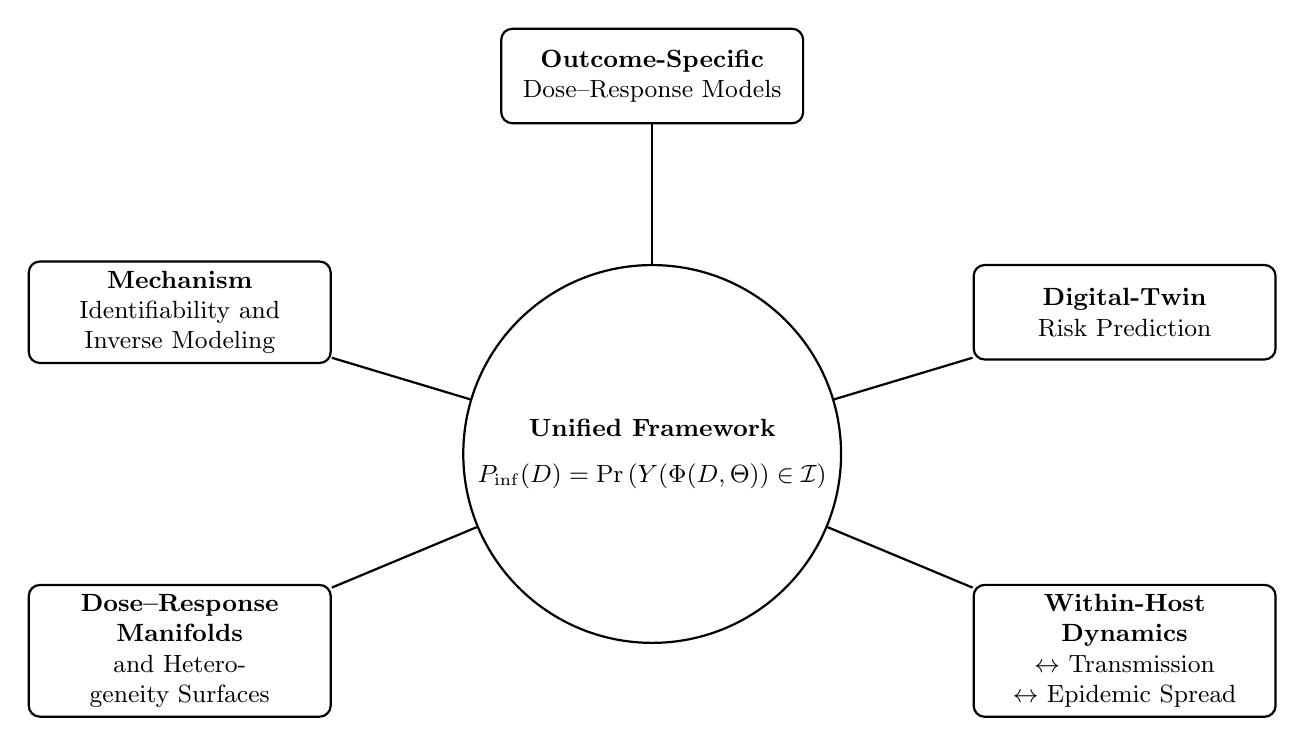
\begin{tikzpicture}[
    font=\small,
    hub/.style={
        circle,
        draw=black,
        thick,
        align=center,
        minimum size=3.8cm
    },
    spoke/.style={
        rectangle,
        rounded corners,
        draw=black,
        thick,
        align=center,
        text width=3.6cm,
        minimum height=1.2cm
    },
    arrow/.style={-, thick}
]

% Central hub
\node[hub] (center) at (0,0)
{
\textbf{Unified Framework}\\[2mm]
$\displaystyle
P_{\mathrm{inf}}(D)
=
\Pr\left(
Y(\Phi(D,\Theta))
\in \mathcal I
\right)$
};

% Top
\node[spoke] (outcome) at (0,4.8)
{
\textbf{Outcome-Specific}\\
Dose--Response Models
};

% Right
\node[spoke] (digital) at (6.0,1.8)
{
\textbf{Digital-Twin}\\
Risk Prediction
};

% Lower right
\node[spoke] (epidemic) at (6.0,-2.5)
{
\textbf{Within-Host Dynamics}\\
$\leftrightarrow$ Transmission\\
$\leftrightarrow$ Epidemic Spread
};

% Lower left
\node[spoke] (manifold) at (-6.0,-2.5)
{
\textbf{Dose--Response Manifolds}\\
and Heterogeneity Surfaces
};

% Left
\node[spoke] (inverse) at (-6.0,1.8)
{
\textbf{Mechanism}\\
Identifiability and\\
Inverse Modeling
};

% Connections
\draw[arrow] (center) -- (outcome);
\draw[arrow] (center) -- (digital);
\draw[arrow] (center) -- (epidemic);
\draw[arrow] (center) -- (manifold);
\draw[arrow] (center) -- (inverse);

\end{tikzpicture}
}

\caption{
Future research directions emerging from the unified dose--response framework. The central formulation,
$P_{\mathrm{inf}}(D)
=
\Pr\left(
Y(\Phi(D,\Theta))
\in \mathcal I
\right)
$,
provides a common mathematical structure linking exposure, biological variability, within-host dynamics, and outcome definitions. The framework naturally motivates several future directions, including outcome-specific dose--response modeling, mechanism identifiability and inverse modeling, dose--response manifolds incorporating biological heterogeneity, individualized risk prediction through digital-twin approaches, and integration of within-host dynamics with transmission and epidemic processes.
}
\label{fig:future_directions_framework}
\end{figure}

The unified framework developed in this review not only provides a common interpretation of existing dose--response models but also suggests several directions for future research. As illustrated in Figure~\ref{fig:future_directions_framework}, the central exposure-to-outcome mapping

\[
P_{\mathrm{inf}}(D)
=
\Pr\left(Y(\Phi(D,\Theta))\in\mathcal I\right)
\]

provides a general mathematical structure linking exposure, biological variability, within-host dynamics, and outcome definitions. This perspective shifts attention from fitting dose--response curves toward understanding the mechanisms that generate them.

One important direction is the development of \emph{outcome-specific dose--response models}. Within the proposed framework, infection represents only one possible outcome criterion. Alternative endpoints may include colonization, symptomatic disease, severe disease, pathogen shedding, or transmission potential. The framework therefore supports a broader class of dose--response relationships tailored to different biological and public-health objectives.

A second opportunity lies in addressing \emph{mechanism identifiability and biological heterogeneity}. Similar dose--response curves may emerge from fundamentally different establishment processes, within-host dynamics, and sources of variability. Future studies may therefore focus on inverse modeling approaches that infer underlying biological mechanisms from observed dose--response patterns. More generally, the explicit representation of host, pathogen, and environmental variability suggests a transition from one-dimensional dose--response curves toward higher-dimensional risk surfaces that characterize heterogeneous biological populations.

Finally, the framework provides a foundation for integrating dose–response processes across scales. Individualized parameterization may support digital-twin approaches for personalized risk prediction, in which mechanistic models are combined with subject-specific physiological and clinical information \cite{Venkatesh2024DigitalTwins}, while coupling within-host dynamics to pathogen shedding and infectiousness may link dose–response models directly to transmission and epidemic spread \cite{Handel2015CrossingScale,Mideo2008WithinHost}. Together, these directions suggest that mechanistic dose--response modeling can serve as a bridge between risk assessment, within-host biology, and population-level infectious disease dynamics. These future directions are summarized schematically in Figure~\ref{fig:future_directions_framework}.


%-----------------------------------------------------------------------------------------------------------------
\section{Computational Demonstration of the Exposure-to-Outcome Framework}\label{sec:computational_demonstration}

%-----------------------------------------------------------------------------------------------
\subsection{Mechanistic model and outcome definition}
\label{sec:illustrative_example}

%To illustrate how dose--response relationships emerge within the proposed framework, we consider a minimal mechanistic model coupling pathogen dynamics with immune activity. These mechanisms are commonly represented in
%within-host infection models \cite{Alizon2009VirulenceReview,Rahman2018AdvancingRiskAssessment}.
%This benchmark model represents one illustrative realization of the unified framework developed in Section~\ref{sec:mechanistic_framework}. Other realizations may employ stochastic establishment processes, branching-process formulations, agent-based models, or multiscale within-host systems. The purpose of the present example is not pathogen-specific realism or calibration, but rather to demonstrate how the key components of the framework—dose-to-state mapping, within-host dynamics, outcome definition, biological variability, and population-level aggregation—combine to generate an emergent dose–response relationship. The particular choices made below are intended solely to provide a transparent and tractable illustration of the framework.


To illustrate how dose--response relationships emerge within
the proposed framework, we revisit the minimal pathogen--immune
model introduced in Section~\ref{path_immune_frame}, Eqs.~\eqref{eq:pathogen_dynamics}--\eqref{eq:immune_dynamics}.
This model provides one illustrative realization of the unified framework developed in Section~\ref{sec:mechanistic_framework}.

The purpose of this example is not pathogen-specific realism
or calibration, but rather to demonstrate how dose-to-state
mapping, within-host dynamics, outcome definition, biological
variability, and population-level aggregation combine to
generate an emergent dose--response relationship.

For convenience, we restate the system
\begin{equation}
\frac{dP}{dt}
=
\lambda P\left(1-\frac{P}{K}\right)
-\phi PI
-\mu P,
\label{eq:example_pathogen}
\end{equation}

\begin{equation}
\frac{dI}{dt}
=
\alpha P
+
\beta I\left(1-\frac{I}{I_{\max}}\right)
-
\delta I,
\label{eq:example_immune}
\end{equation}
where $P(t)$ denotes pathogen burden and $I(t)$ denotes immune activity.
The parameter $\lambda$ controls pathogen replication,
$K$ is the within-host carrying capacity,
$\phi$ represents immune-mediated clearance,
and $\mu$ denotes baseline pathogen loss.
Immune activation is governed by $\alpha$,
while $\beta$ and $\delta$ describe immune expansion and decay, respectively.

Exposure dose enters the system through the dose-to-state mapping
\begin{equation}
P(0)=\eta D,
\label{eq:example_initial}
\end{equation}
where $D$ denotes the external inoculum dose and $\eta$ represents the fraction of pathogens surviving early physiological and environmental barriers.
Initial immune activity is specified as
\begin{equation}
I(0)=I_0.
\end{equation}


%Infection outcomes are defined through threshold crossing of pathogen burden.
%Let
%\begin{equation}
%Y(D,\Theta)
%=
%\max_{0\le t\le T} P(t;D,\Theta),
%\end{equation}
%where $\Theta$ denotes host-specific biological parameters and $T$ is the
%observation horizon. Infection is defined by the event
%\begin{equation}
%\mathcal{I}
%=
%\{Y(D,\Theta)\ge P_c\},
%\label{eq:infection_threshold_example}
%\end{equation}
%where $P_c$ denotes the pathogen establishment threshold.


%{\bf fffffffff}
The following derivation illustrates how an effective establishment
criterion and a corresponding operational infection threshold can be
obtained from the local balance between pathogen growth and immune-mediated
clearance. 

During the early within-host phase, the local growth
or decline of pathogen burden depends on the balance
between pathogen replication and immune-mediated
clearance. For small pathogen burden ($P\ll K$), Eq.~\eqref{eq:example_pathogen}
reduces to
\begin{equation}
\frac{dP}{dt}
\approx
(\lambda-\phi I-\mu)P.
\end{equation}

This motivates the effective within-host establishment number
\begin{equation}
\mathcal{R}_{\mathrm{est}}(t)
=
\frac{\lambda}{\phi I+\mu},
\label{eq:Rest}
\end{equation}
which serves as an effective within-host establishment criterion analogous
to a reproduction threshold. Under the low-burden approximation, pathogen burden
increases locally when
\begin{equation}
\mathcal{R}_{\mathrm{est}}(t)>1,
\end{equation}
whereas
\begin{equation}
\mathcal{R}_{\mathrm{est}}(t)<1
\end{equation}
indicates a local decline in pathogen burden.
Since $\mathcal{R}_{\mathrm{est}}(t)$ depends on the
time-varying immune response, these conditions
characterize instantaneous pathogen growth or
decline rather than determining the long-term
infection outcome.


Operationally, infection outcomes are classified using the event
\begin{equation} 
\mathcal{E} =
\left\{
\max_{0 \le t \le T} P(t;D,\Theta)\ge P_c
\right\}.
\label{eq:infection_threshold_example}
\end{equation}
where $P_c$ denotes a detectable or biologically meaningful pathogen
burden threshold.



The low-burden growth-neutral condition
$R_{\mathrm{est}}(t)=1$ yields the critical
immune activity
\begin{equation}
I_c=\frac{\lambda-\mu}{\phi}.
\end{equation}
To relate this condition to a pathogen burden threshold, we evaluate the
immune nullcline from Eq.~\eqref{eq:example_immune},
\begin{equation}
\alpha P+\beta I\left(1-\frac{I}{I_{\max}}\right)-\delta I=0.
\end{equation}
Setting $I=I_c$ gives the corresponding critical pathogen burden
\begin{equation}
P_c^{\ast}
=
\frac{
\delta I_c
-
\beta I_c\left(1-\frac{I_c}{I_{\max}}\right)
}{\alpha}.
\end{equation}
Equivalently,
\begin{equation}
P_c^{\ast}
=
\frac{1}{\alpha}
\left[
\frac{\lambda-\mu}{\phi}
\left\{
\delta
-
\beta\left(
1-\frac{\lambda-\mu}{\phi I_{\max}}
\right)
\right\}
\right].
\end{equation}


The quantity $P_c^*$ provides a nullcline-based
reference burden under the low-burden approximation.
It is biologically meaningful when
$0<I_c<I_{\max}$ and $P_c^*>0$.

%This expression provides a mechanistically motivated reference burden
%associated with the transition between pathogen expansion and immune-mediated
%clearance under the local equilibrium approximation. The reference threshold is
%biologically meaningful when $0<I_c<I_{\max}$ and $P_c^{\ast}>0$.
%%Thus, $P_c^{\ast}$ provides a mechanistic reference threshold for
%%infection establishment.
%Thus, $P_c^*$ provides a nullcline-based reference
%burden associated with the local balance between
%pathogen growth and immune activity.

For the illustrative simulations, we use the operational threshold
\begin{equation}
P_c=\rho K,\qquad 0<\rho<1.
\end{equation}
Here, $\rho$ specifies the fraction of the
within-host carrying capacity used as an
operational positive-response classification threshold.
Unless otherwise stated, we take $\rho=10^{-2}$,
corresponding to a pathogen burden equal to
one percent of the carrying capacity.

%where $\rho$ represents the fraction of the pathogen carrying capacity
%associated with successful establishment or detectable infection. This
%choice ensures a positive and interpretable threshold while retaining the
%mechanistic interpretation that infection corresponds to trajectories
%crossing an establishment boundary. Unless otherwise stated, we take
%$\rho=10^{-2}$, corresponding to trajectories reaching one percent of the
%within-host carrying capacity.


The reference burden $P_c^*$ is obtained from the
intersection of the immune nullcline with the
low-burden pathogen growth-neutral condition.
It should not, in general, be interpreted as a
dynamical separatrix or a rigorous threshold for
infection establishment. In contrast, the operational
threshold $P_c=\rho K$ is prescribed independently
to classify within-host trajectories according to
whether pathogen burden reaches a specified level
during the observation interval. Consequently, the
resulting dose--response curve represents the
population-level probability of finite-time threshold
crossing under heterogeneous biological parameters,
rather than the probability of avoiding stochastic
extinction.

%For the nominal parameter set, the pathogen-free
%equilibrium is unstable to pathogen invasion,
%indicating that the illustrative system permits
%persistent pathogen dynamics. Accordingly,
%the dose--response outcome is defined through
%finite-time crossing of the operational burden
%threshold rather than asymptotic pathogen clearance.


To represent host heterogeneity, selected parameters are treated as random variables and the variability vector $\Theta$ is restricted to the parameters $(\eta, \phi)$. In particular, variability in survival through early barriers and immune-mediated clearance is modeled through
\begin{equation}
\eta \sim \mathrm{Lognormal}(\mu_\eta,\sigma_\eta^2),
\qquad
\phi \sim \mathrm{Lognormal}(\mu_\phi,\sigma_\phi^2).
\label{eq:example_variability}
\end{equation}

For each dose level, virtual hosts are generated by sampling parameter
realizations from Eq.~\eqref{eq:example_variability}. The within-host
system is solved over the interval $[0,T]$, and infection outcomes are
classified according to Eq.~\eqref{eq:infection_threshold_example}. The resulting population-level finite-time threshold-crossing probability is estimated as
\begin{equation}
\widehat{P}_{\mathrm{cross}}(D)
=
\frac{1}{N}
\sum_{i=1}^N
\mathbf{1}
\left[
\max_{0\le t\le T} P_i(t)\ge P_c
\right].
\label{eq:estimated_dose_response}
\end{equation}
where $\mathbf{1}_{\{\cdot\}}$ denotes the indicator function.

This construction illustrates several central features of the mechanistic framework.
First, exposure dose determines initial within-host conditions rather than infection probability directly.
Second, infection outcomes emerge from the resulting biological trajectories generated by Eqs.~\eqref{eq:example_pathogen}--\eqref{eq:example_immune}.
Third, population-level dose--response curves arise only after aggregation across heterogeneous hosts.
The illustrative calculation produces a dose-dependent threshold-crossing response. It does not demonstrate that the exponential or Beta--Poisson formulas can be derived from this particular pathogen--immune system; such reductions require separate mathematical assumptions or model comparisons.

%-------------------------------------------------------------------
\subsection{Simulation design}


Using the mechanistic framework introduced above,
we performed Monte Carlo simulations of
heterogeneous deterministic within-host trajectories
to illustrate the generation of population-level
dose--response relationships.

%Using the mechanistic framework introduced above, we performed stochastic within-host simulations to illustrate how heterogeneous biological trajectories generate emergent dose--response relationships.

Exposure doses were logarithmically spaced over the range
\[
10^0 \text{--} 10^8.
\]
For each exposure level, dose was mapped to initial pathogen burden through Eq.~\eqref{eq:example_initial}.
Host heterogeneity was incorporated by sampling the survival parameter $\eta$ and immune-clearance parameter $\phi$ from the lognormal distributions defined in Eq.~\eqref{eq:example_variability}.

Unless otherwise stated, simulations used
\[
\lambda=1.0,\quad
K=10^8,\quad
\phi=2\times10^{-5},\quad
\mu=0.1,
\]
\[
\alpha=10^{-3},\quad
\beta=0.3,\quad
I_{\max}=10^5,\quad
\delta=0.2,
\]
with initial immune activity
\[
I(0)=4\times10^4.
\]

The survival parameter $\eta$ was assigned logarithmic standard deviation $\sigma_\eta=0.4$, while the immune-clearance parameter $\phi$ was assigned logarithmic standard deviation $\sigma_\phi=0.25$. The corresponding lognormal location parameters were
$\mu_\eta=\ln(10^{-3})-\sigma_\eta^2/2
\approx -6.99$ and
$\mu_\phi=\ln(2\times10^{-5})-\sigma_\phi^2/2
\approx -10.85$,
yielding arithmetic means
$\mathbb{E}[\eta]=10^{-3}$ and
$\mathbb{E}[\phi]=2\times10^{-5}$.


Simulations were performed over the interval
\[
t\in[0,30]
\]
using $N=300$ virtual hosts per dose and $M=100$ repeated Monte Carlo realizations. At each dose, the central estimate was the median of the $M=100$ replicate proportions, and the plotted 95\% Monte Carlo percentile interval used their empirical 2.5th and 97.5th percentiles. This interval describes variation in finite-host Monte Carlo estimates under the prescribed host-parameter distributions; it is neither a confidence interval for biological parameter uncertainty nor a predictive interval for an individual host.



The simulations used 12 logarithmically spaced doses and independent lognormal draws of $\eta$ and $\phi$ for each virtual host in each repetition. A NumPy pseudorandom seed of 123 was set at the beginning of the computation. The coupled ordinary differential equations were integrated with SciPy's \texttt{solve\_ivp} using the explicit RK45 solver, relative tolerance $10^{-6}$ and absolute tolerance $10^{-9}$. Each trajectory was evaluated at 400 equally spaced times over $[0,30]$; the recorded maximum over those sampled times determined the threshold-crossing indicator. Therefore, the implemented outcome is a sampled-time approximation to the continuous-time maximum in Eq.~\eqref{eq:estimated_dose_response}. A crossing that occurs and reverses between output times could be missed; continuous event detection would remove this numerical limitation. Solver success was not explicitly checked in the original scripts, so reproducibility should include a solver-success check before publication.

Repeated Monte Carlo realizations were used to characterize finite-sample variability in
the estimated population-level infection probability under the specified distributions
of heterogeneous host parameters.
%
%Dose–response curves were generated using the estimator defined in Eq.~\eqref{eq:estimated_dose_response}. Repeated Monte Carlo realizations were used to characterize the variability in population-level infection probability arising from heterogeneous parameter values across virtual hosts. 
%------------------------------------------------------

\begin{figure}[H]
\centering
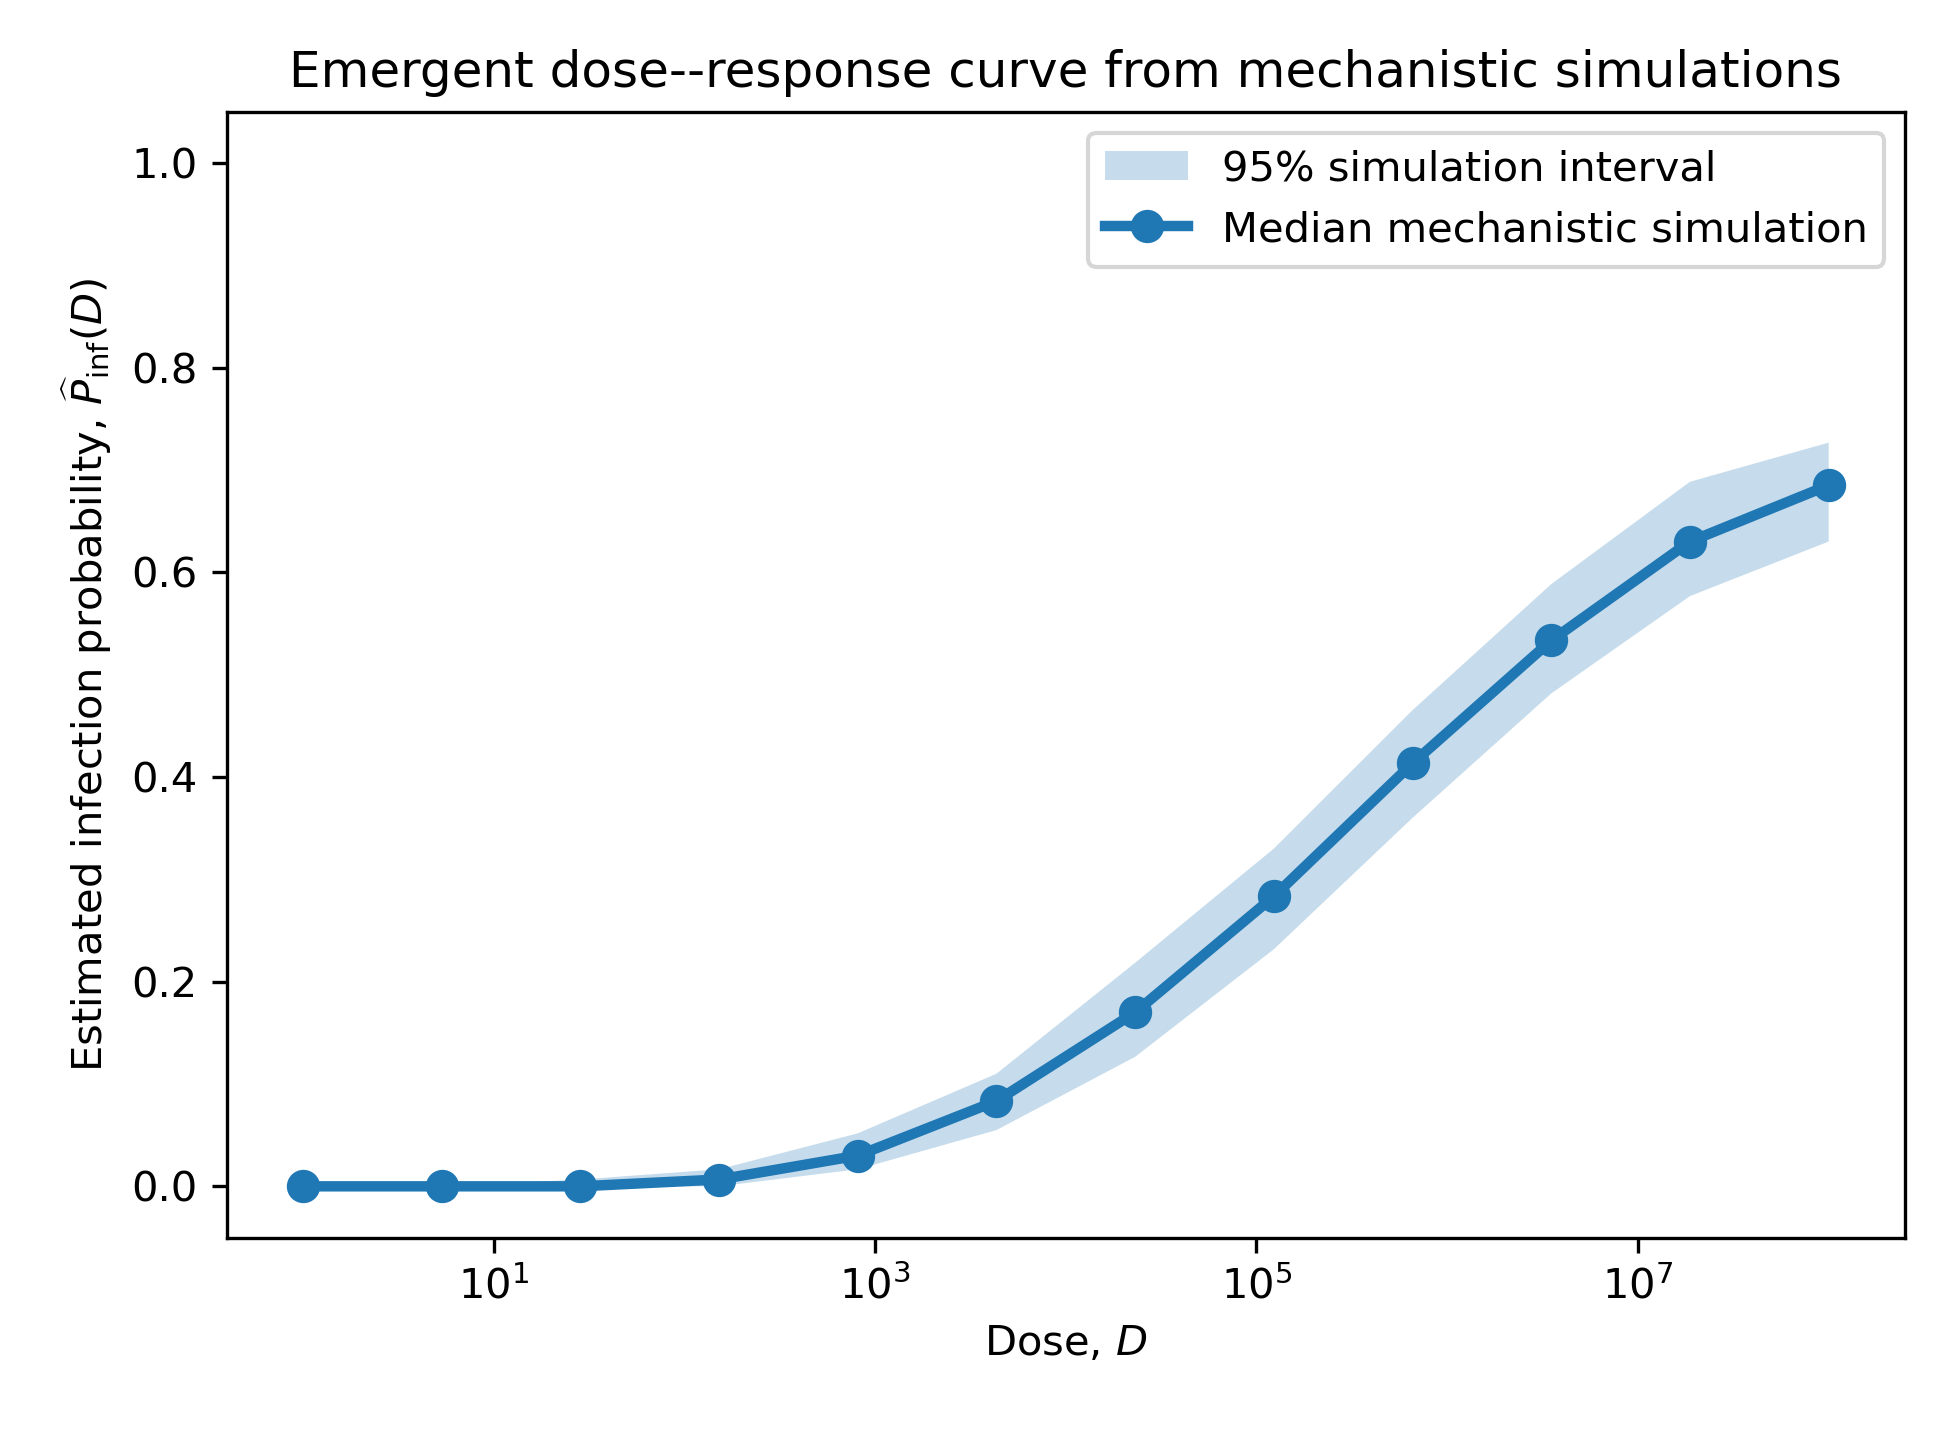
\includegraphics[width=0.78\textwidth]{dose_response_curve_with_band.png}
\caption{
Emergent dose--response relationship generated from the mechanistic
within-host framework. The finite-time threshold-crossing response was estimated by
aggregating binary outcomes across heterogeneous virtual
hosts with variable survival and immune-response parameters.
The line is the median of 100 replicate estimates (300 virtual hosts per dose); shading shows the 2.5th--97.5th percentile range of those replicate estimates, not biological predictive uncertainty.
}
\label{fig:mechanistic_dose_response}
\end{figure}
%%%%%%%%%%%%%%-------------------------------------------------
\subsection{Simulation results}

The simulations illustrate how population-level dose--response
relationships can emerge from heterogeneous within-host dynamics.
Figure~\ref{fig:mechanistic_dose_response} shows the estimated
threshold-crossing probability across exposure doses obtained from repeated
Monte Carlo realizations of the mechanistic model.


At low exposure doses, trajectories generally remain below
the operational threshold during the observation period.
Intermediate doses produce mixed outcomes, including both
sub-threshold and threshold-crossing trajectories depending
on host-specific parameters. At sufficiently high doses,
trajectories more consistently exceed the operational
threshold and reach elevated pathogen burdens. As dose
increases, threshold-crossing events become more frequent,
producing a gradual nonlinear increase in the estimated
positive-response probability. The shaded region represents
the 95\% Monte Carlo percentile interval, calculated from
repeated estimates of the population-level response
probability. This interval reflects finite-sample variability
in the Monte Carlo estimates under the prescribed
distributions of host-specific survival and immune-response
parameters.


The displayed trajectories are the first four sampled hosts at each of three selected doses from the first Monte Carlo repetition, rather than averages or typical quantiles. The corresponding within-host trajectories are shown in
Figure~\ref{fig:trajectory_examples}. At low exposure doses,
trajectories generally remain below the operational threshold
during the observation period. Intermediate doses produce
mixed outcomes, with some trajectories remaining below
the threshold and others crossing it, depending on
host-specific parameters. At sufficiently high doses,
trajectories more consistently exceed the operational
threshold and reach elevated pathogen burdens.


\begin{figure}[ht]
\centering
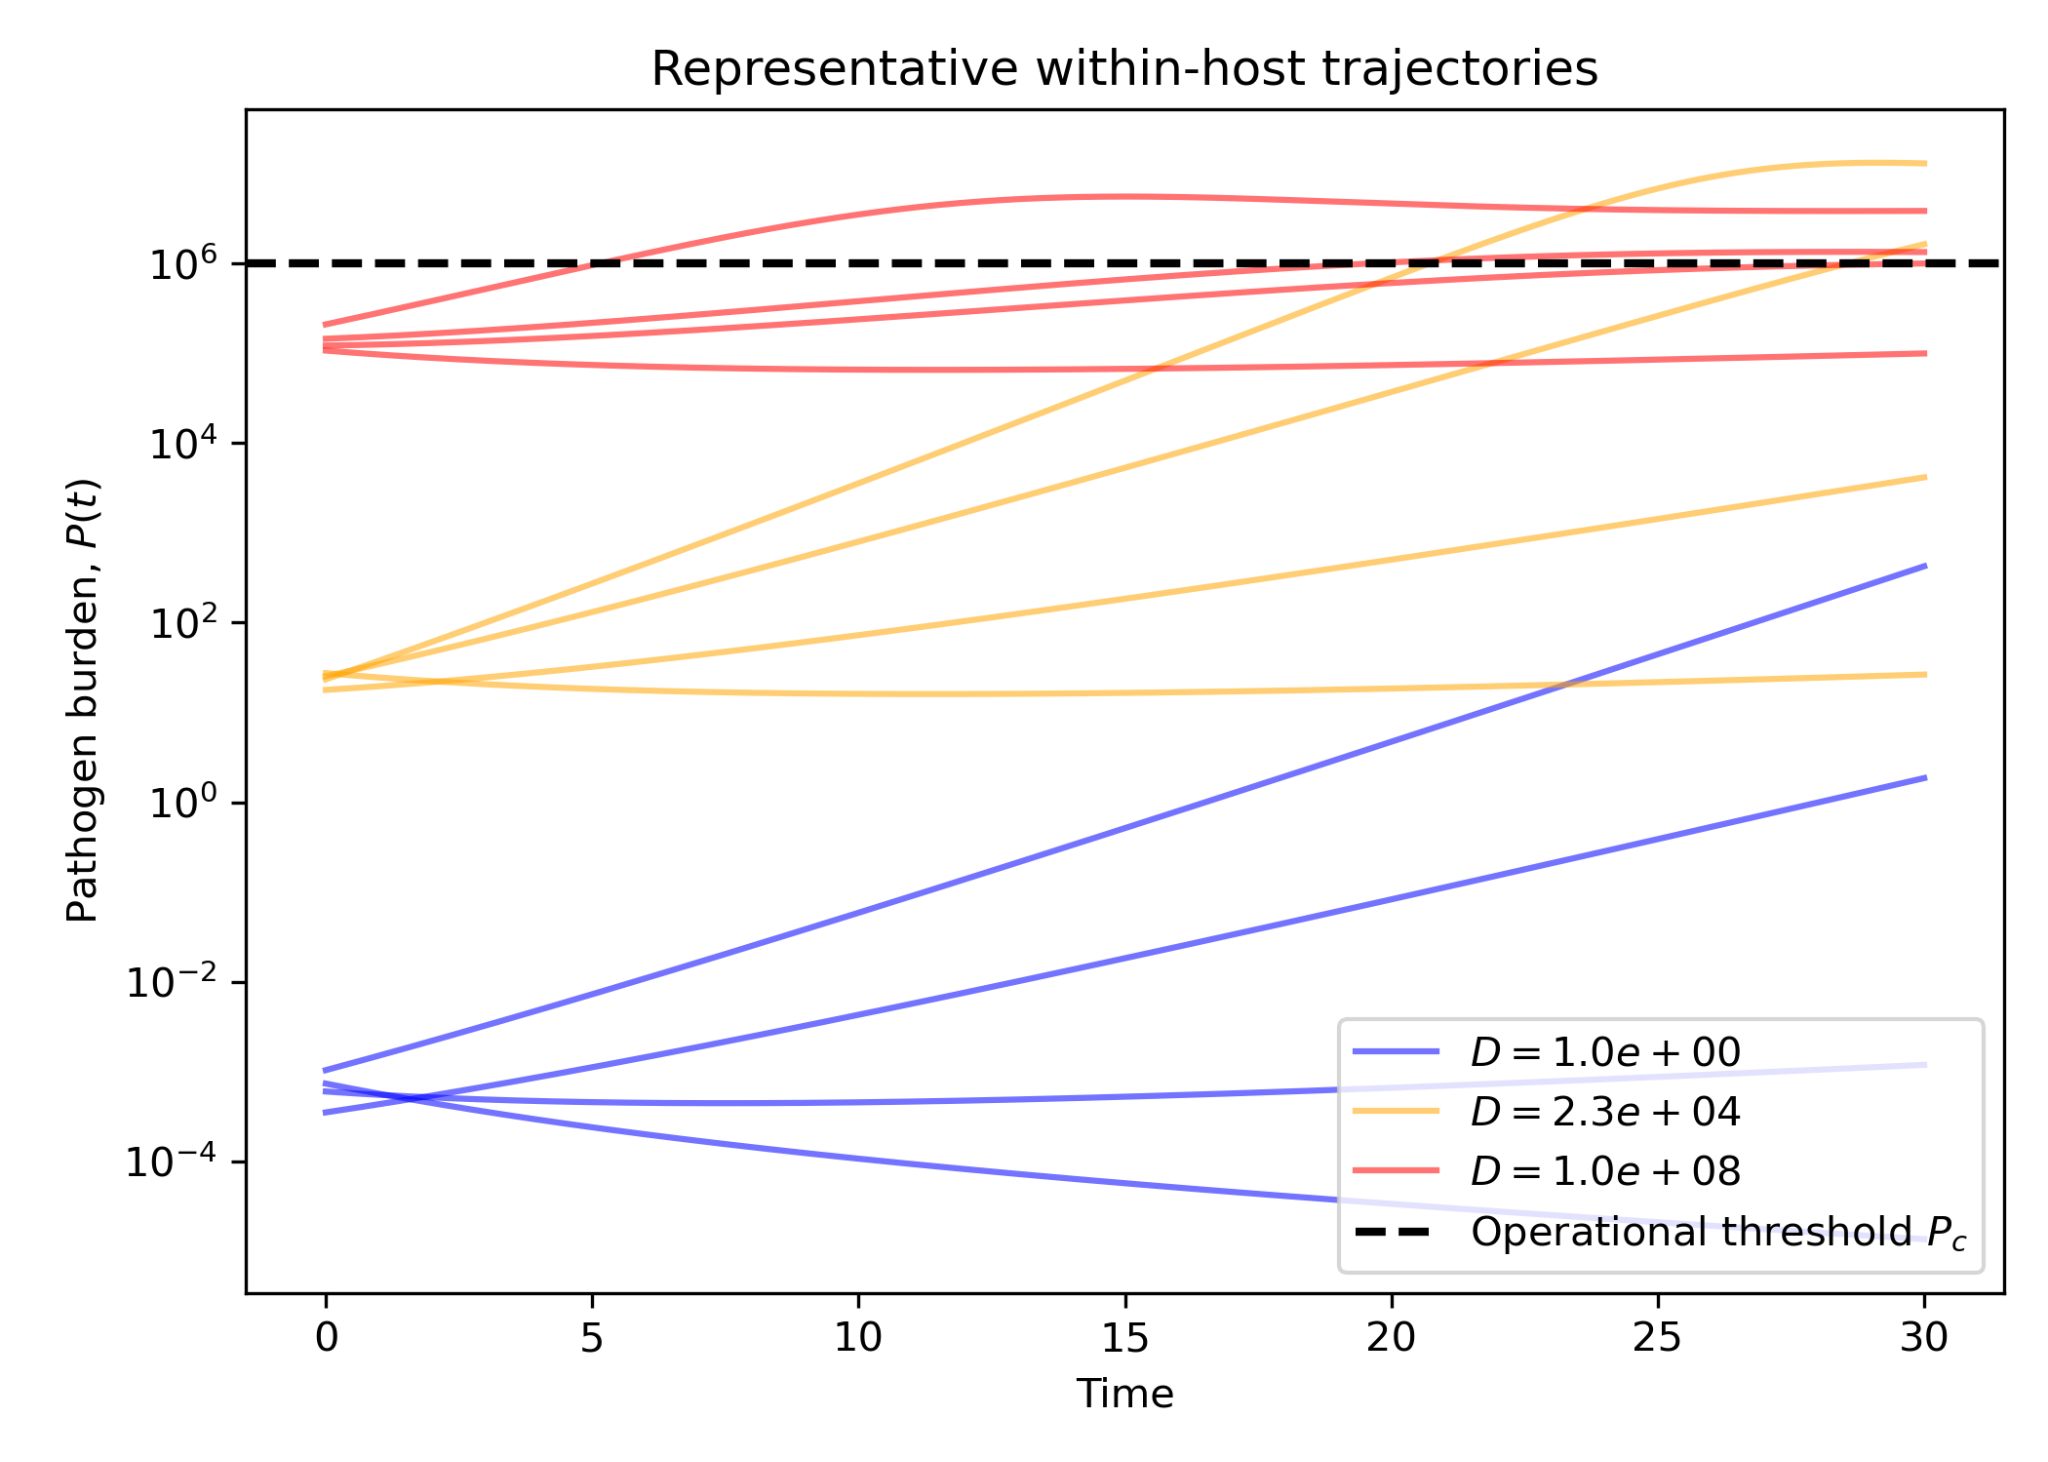
\includegraphics[width=0.78\textwidth]{trajectory_examples.png}
\caption{Representative within-host pathogen trajectories
generated by the mechanistic model across illustrative
exposure doses ($D=1$, $D\approx 2.3\times 10^4$, and $D=10^8$). Four trajectories are shown per dose from the first Monte Carlo repetition. The dashed horizontal line denotes the
operational threshold $P_c=\rho K$. At low doses,
trajectories generally remain below this threshold during
the observation period, whereas higher doses more
frequently produce threshold-crossing trajectories.
Crossing the operational threshold indicates a positive
response within the observation interval and does not
necessarily imply permanent infection establishment.}
\label{fig:trajectory_examples}
\end{figure}

Together, these simulations illustrate the central premise of the
proposed framework: dose--response curves can be interpreted as
emergent properties of heterogeneous within-host dynamics rather than
as imposed empirical mappings. In this illustration, population-level
threshold-crossing probabilities arise through aggregation of heterogeneous
host trajectories shaped by pathogen growth, immune dynamics,
threshold behavior, and biological variability.

The current illustrative model supports a
mathematically well-defined probability of
finite-time pathogen-burden threshold crossing. However, under the nominal parameter values,
it does not demonstrate a stable
clearance-versus-establishment transition. A future extension could investigate alternative
parameter regimes, nonlinear immune-response
mechanisms, bistability, and stochastic extinction
to develop a more biologically explicit
infection-establishment criterion.

\section{Conclusion}
\label{sec:conclusion}

Mechanistic dose--response modeling is most useful when viewed not as a single class of models but as a unifying framework that links exposure, pathogen biology, and host processes to measurable outcomes. Within this perspective, dose--response relationships are not treated as purely empirical curves, but as emergent properties of pathogen survival, within-host dynamics, and biological variability.

This perspective clarifies how classical, mechanistic, and hybrid approaches relate within a common structure. Classical models provide parsimonious summaries of infection risk under limited data, whereas mechanistic and stochastic models explicitly represent the biological processes governing infection establishment and progression. Hybrid and multiscale approaches extend this structure by integrating within-host dynamics, heterogeneity, and data-driven components, enabling more flexible and scalable analysis. As illustrated in Figure~\ref{fig:future_directions_framework}, these approaches form a continuum from descriptive to process-based representations of risk.

The principal contribution of this work is the development of a unified conceptual and mathematical formulation that links exposure to infection through a common mechanistic mapping. This formulation enables consistent interpretation, comparison, and extension
of existing models across different levels of biological detail and modeling
paradigms, while making explicit where biological variability and uncertainty
enter and propagate through the exposure-to-outcome pathway. %This formulation enables consistent interpretation, comparison, and extension of existing models across different levels of biological detail and modeling paradigms, and provides a direct pathway for integrating biologically grounded infection processes into epidemic models.

Despite these advances, important challenges remain in data availability, parameter identifiability, and model validation. Addressing these challenges will require tighter integration of experimental, epidemiological, and high-dimensional biological data, together with continued advances in stochastic modeling and scientific machine learning. At the same time, effective models must balance biological realism with tractability to ensure interpretability and practical applicability.

The framework is intentionally general and is not tied to a specific pathogen. The numerical demonstration produces a finite-time pathogen-burden threshold-crossing probability, not a validated probability of permanent infection or clinical disease. No pathogen-specific observations were used to calibrate or validate the illustrative parameterization. Future work should test the framework against observed infection endpoints, compare its predictions with fitted classical models, and assess parameter identifiability and predictive uncertainty.



%-------------------------------------------------------------------
\section*{Data availability}
No empirical datasets were generated or analysed. The computational results were produced from simulated virtual-host parameter draws. The numerical code and output workbooks accompanying the revised manuscript reproduce the reported simulation design; these files should be deposited as supplementary information or in a persistent public repository before submission. No public repository is claimed here.

\section*{Code availability}
The accompanying Python scripts specify the model, random-number seed, parameter distributions, solver settings, Monte Carlo repetitions and plotting steps. The final banded-curve script is \texttt{dose-response\_update\_band(1).py}. Before publication, an archived, versioned copy should be made accessible with the numerical outputs.

\section*{Author contributions}

Ashrafur Rahman: Conceptualization, Methodology,
Formal analysis, Software, Investigation,
Visualization, Writing -- original draft,
Writing -- review \& editing.
\section*{Funding}

This research received no specific grant from any
funding agency in the public, commercial, or
not-for-profit sectors.
\section*{Competing interests}
The author declares no conflict of interest.

\section*{Acknowledgments}
The author acknowledges the foundational literature in microbial risk assessment, within-host infectious disease modeling, and host--pathogen dynamics that has made this synthesis possible.

\section*{Declaration of Generative AI and AI-Assisted Technologies in the Manuscript Preparation Process}

During the preparation of this work, the author used ChatGPT (OpenAI) to assist with language editing, improving clarity and organization, and refining the presentation of the manuscript. The author reviewed and edited the output as needed and takes full responsibility for the content of the published article.

\bibliographystyle{unsrtnat}
\bibliography{mechanistic_dose_response_unified_framework}
\end{document}
